\documentclass[12pt,a4paper]{article}
\usepackage{hyperref}
\usepackage{graphicx}
\title{Laboratory 2: Unauthorized Access in Wireless Networks}
\author{Niclas Scheuing and Vasileios Dimitrakis}
\begin{document}
	\maketitle
	
	\section{Introduction}
	The goal of this laboratory exercise is to introduce us to the spread spectrum techniques. Spread spectrum refers to a system developed to spread the signal over a large frequency band, in order to increase the security of the communication. The main idea behind this systems is to use more bandwidth and at the same time to maintain the same amount of power in the whole signal. These techniques offer increased resistance to interference, noise, jamming and channel multipath and fading effects. These properties make them very popular and frequently preferred in communication systems. 
	There are three main spread spectrum techniques that are frequently used:
	\begin{itemize}
	\item{\emph{Frequency Hop Spread Spectrum}: Is a method of transmitting radio signals by rapidly switching a carrier among many frequency channels, using a pseudorandom sequence known to both transmitter and receiver.}
	\item{\emph{Chirp}: Is a signal, which decreases or increases its frequency continuously over time. It has many applications and one of them is the property of spread spectrum that offers.}
	\item{\emph{Direct Sequence Spread spectrum}: Is a spread spectrum technique whereby the original data signal is multiplied with a pseudo random noise spreading code.}
	\end{itemize}
	
	In this exercise we will study the case of the Direct Sequence Spread Spectrum (DSSS).
	In DSSS the signal is used to modulate a bit sequence, which is known as Pseudo Noise (PN) code. This code consists of pulses that have much shorter duration than the one of original signal. Therefore, this process chops up the pulses of the message signal and this leads to broader signal's bandwidth that tends to be equal to the one of the PN code. 
	This spread spectrum technique is widely used, because it offers many benefits and for this reason, it is widely used in both military and civilian communication systems.
	
	\begin{itemize}
	\item{Resistance to intended or unintended jamming.}
	\item{Multiple users can share the same channel.}
	\item{Robust against noise.}
	\item{It provides a way to determine relative timing between transmitter and receiver.}
	\item{DSSS spreads the signal over a wide range of frequency and the latter can be hidden below noise level.}
	\end{itemize}
	
	\section{Topology}
	In this exercise we have one DSSS transmitter and one DSSS receiver. In this system, we have two main signal components: the message signal m(t) and the pseudorandom code code(t). \newline
	\textbf{Transmitter:} First of all, the transmitter modulates the data signal with a primary modulator using a modulation scheme, e.g BPSK. After that it multiplies the outcome of the previous process with the PN code generator and the bandwidth of the signal is spread to a wider range of frequencies.
	\newline
	\textbf{Receiver:} On the other hand, in the receiver the reverse process is followed. Firstly, the receiver despreads the broadened signal using the appropriate PN code. In the next step, it demodulates the signal using the carrier, in order to retrieve the data.
	
	\section{Materials and Methods}
	Throughout the lab exercise 2 we used \emph{MATLAB}, a vector- and numerical computing environment.
		
	\section{Tasks}
		After fixing the code and make it use the same key for spreading and despreading, we executed to following steps:
		\begin{enumerate}
			\item \emph{Configuring the DSSS system}. We set the \texttt{data} array to \texttt{[1 -1 1 -1 1 -1 1 -1 ]} choosing a length that is a multiple of 5. We also choose a code length of 10 bits. These results in a one chip per symbol modulation.
			
			
		\end{enumerate}
	
	\section{Questions}
		\subsection{System configuration}
			Length of message
			Length of code
			chips per symbol \newline
			\textbf{Processing gain:} In a spread spectrum system, the process gain (or 'processing gain') is the ratio of the spread (or RF) bandwidth to the despread (or baseband) bandwidth. It is usually expressed in decibels (dB).
			
		\subsection{Jamming resistance of DSSS}
			Below noise
			multiband
			
		\subsection{Security introduced by DSSS}
		
		\subsection{}
	
	
	\begin{figure}
		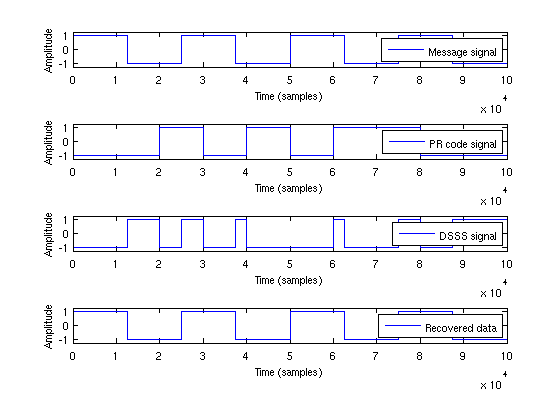
\includegraphics[width=\textwidth]{images/code_cl10_dl10.png}
		\caption{Capturing the traffic using source \emph{MAC} address filtering.}
		\label{wep:wireshark}
	\end{figure}
	
	\section{Analysis}
	In this lab we demonstrated that some widely used security mechanisms as MAC-filtering, WEP and WPA2 are prone to rather simple 
	
	
	\bibliographystyle{plain}
	\bibliography{bibliography}
\end{document}\grid
